\documentclass{article}

\usepackage[margin=0.75in]{geometry}
\usepackage{graphicx}
\usepackage{amsmath}
\usepackage{float}
\usepackage[hidelinks]{hyperref}

\begin{document}

\title{Short Report: Independent Smooth Signed Radial Kernel}
\author{}
\date{9 April 2026}
\maketitle
\footnotesize
\setlength{\parindent}{0pt}
\setlength{\parskip}{0.35em}

\section*{Objective}

The last training cell replaces the earlier seed-dependent radial fit with an independent radial kernel learned from scratch. The goal is to make the learned kernel shape matter more directly, while keeping the profile stable and interpretable. The final cell after it is only a compact presentation cell: it shows the learned kernel, the final radial profile, and the validation curve for reporting.

\section*{Approach}

The kernel is still radial, so it is represented by one value per radius shell,
\[
K(x,y)=\sum_{r=0}^{R} f_r\,B_r(x,y),
\]
but the new profile is not initialized from the previously trained kernel. Instead, it starts from a generic decaying curve and learns the shell values through a monotone parameterization. The optimization variable is a positive shell-difference vector; cumulative summation then produces a profile that is automatically nonnegative and nonincreasing. The profile is normalized to unit \(\ell_2\) norm at every step, so the optimizer cannot improve the score merely by inflating the kernel magnitude.

This cell also changes the patch score. Rather than using \texttt{abs\_max}, it computes a signed top-\(k\) mean response: the convolution map is formed, the locations with the largest absolute responses are selected, and their signed values are averaged. This is the key change that makes the radial shape more important. A large response must now be both strong and sign-consistent across several important locations, instead of being dominated by one absolute peak.

To keep the learned profile smooth and physically reasonable, the loss adds four structural penalties on top of the classification loss:
\begin{itemize}
    \item first-difference smoothing, which discourages abrupt shell-to-shell jumps,
    \item second-difference curvature regularization, which discourages isolated spikes,
    \item radial decay regularization, which suppresses large weights at large radii,
    \item an edge penalty on the last shell, which pushes the outer tail toward zero.
\end{itemize}

After training, the same cell calibrates the signed feature with logistic regression and then computes an exact patch-level heatmap on a sliding grid. That heatmap is consistent with the signed training score rather than with an \texttt{abs\_max} surrogate.

\section*{Interpretation}

The practical meaning of this design is simple. The method still keeps the radial inductive bias, but it removes the main shortcuts that previously made the kernel less identifiable. The profile cannot grow arbitrarily, the outer shells are discouraged from becoming active, and isolated spikes are penalized. At the same time, the signed top-\(k\) aggregation makes discrimination depend more on the learned signed radial pattern itself, not just on the magnitude of one response maximum.

\begin{figure}[H]
    \centering
    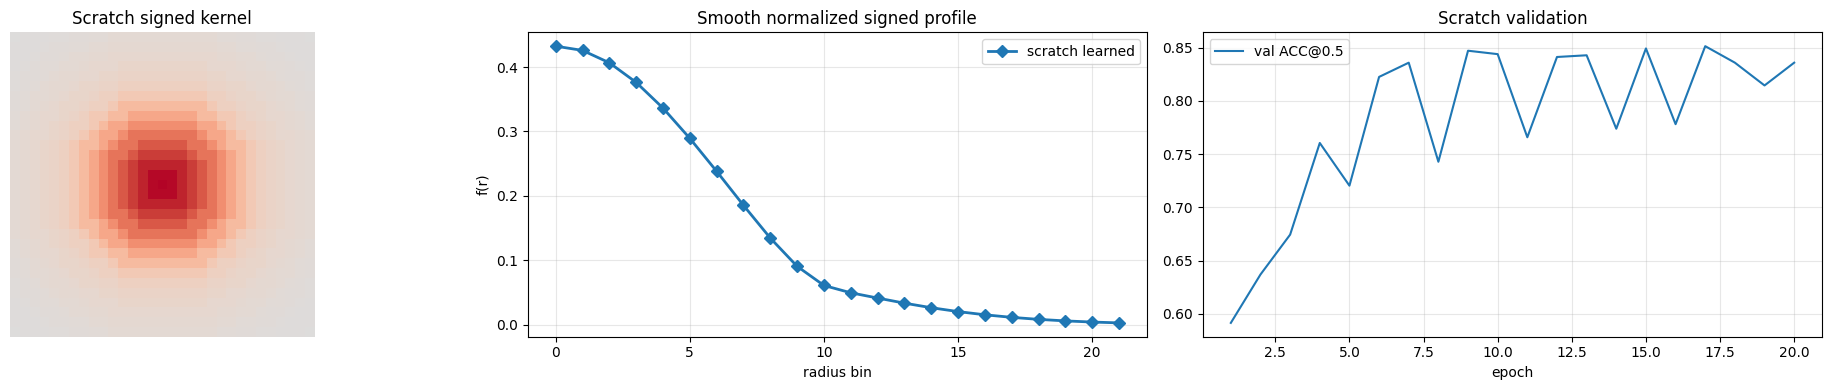
\includegraphics[width=\textwidth]{figures/radial_single_kernel_scratch_summary.png}
    \caption{Compact summary from the final cell: learned signed radial kernel, final smooth normalized profile, and validation accuracy curve.}
\end{figure}

\end{document}
